\documentclass[xcolor={dvipsnames}]{beamer}
%\usepackage[utf8]{inputenc}
%\usetheme{Madrid}
\usetheme{CambridgeUS}
%\usetheme{Malmoe}
%\usecolortheme{beaver}
\usecolortheme{seahorse}

%-------------------------------------------------------------------------------
%          -Packages nécessaires pour écrire en Français et en UTF8-
%-------------------------------------------------------------------------------
\usepackage[utf8]{inputenc}
\usepackage[frenchb]{babel}
\usepackage[T1]{fontenc}
\usepackage{lmodern}
\usepackage{textcomp}

%-------------------------------------------------------------------------------

%-------------------------------------------------------------------------------
%                          -Outils de mise en forme-
%-------------------------------------------------------------------------------
\usepackage{hyperref}
\hypersetup{pdfstartview=XYZ}
\usepackage{enumerate}
\usepackage{graphicx}
%\usepackage{multicol}
%\usepackage{tabularx}

%\usepackage{anysize} %%pour pouvoir mettre les marges qu'on veut
%\marginsize{2.5cm}{2.5cm}{2.5cm}{2.5cm}

\usepackage{indentfirst} %%pour que les premier paragraphes soient aussi indentés
\usepackage{verbatim}
%\usepackage[table]{xcolor}  
%\usepackage{multirow}
\usepackage{ulem}
%-------------------------------------------------------------------------------


%-------------------------------------------------------------------------------
%                  -Nécessaires pour écrire des mathématiques-
%-------------------------------------------------------------------------------
\usepackage{amsfonts}
\usepackage{amssymb}
\usepackage{amsmath}
\usepackage{amsthm}
\usepackage{tikz}
\usepackage{xlop}
\usepackage[output-decimal-marker={,}]{siunitx}
%-------------------------------------------------------------------------------


%-------------------------------------------------------------------------------
%                    - Mise en forme 
%-------------------------------------------------------------------------------

\newcommand{\bu}[1]{\underline{\textbf{#1}}}


\usepackage{ifthen}


\newcommand{\ifTrue}[2]{\ifthenelse{\equal{#1}{true}}{#2}{$\qquad \qquad$}}

\newcommand{\kword}[1]{\textcolor{red}{\underline{#1}}}


%-------------------------------------------------------------------------------



%-------------------------------------------------------------------------------
%                    - Racourcis d'écriture -
%-------------------------------------------------------------------------------

% Angles orientés (couples de vecteurs)
\newcommand{\aopp}[2]{(\vec{#1}, \vec{#2})} %Les deuc vecteurs sont positifs
\newcommand{\aopn}[2]{(\vec{#1}, -\vec{#2})} %Le second vecteur est négatif
\newcommand{\aonp}[2]{(-\vec{#1}, \vec{#2})} %Le premier vecteur est négatif
\newcommand{\aonn}[2]{(-\vec{#1}, -\vec{#2})} %Les deux vecteurs sont négatifs

%Ensembles mathématiques
\newcommand{\naturels}{\mathbb{N}} %Nombres naturels
\newcommand{\relatifs}{\mathbb{Z}} %Nombres relatifs
\newcommand{\rationnels}{\mathbb{Q}} %Nombres rationnels
\newcommand{\reels}{\mathbb{R}} %Nombres réels
\newcommand{\complexes}{\mathbb{C}} %Nombres complexes


%Intégration des parenthèses aux cosinus
\newcommand{\cosP}[1]{\cos\left(#1\right)}
\newcommand{\sinP}[1]{\sin\left(#1\right)}

%Fractions
\newcommand{\myfrac}[2]{{\LARGE $\frac{#1}{#2}$}}

%Vocabulaire courrant
\newcommand{\cad}{c'est-à-dire}

%Droites
\newcommand{\dte}[1]{droite $(#1)$}
\newcommand{\fig}[1]{figure $#1$}
\newcommand{\sym}{symétrique}
\newcommand{\syms}{symétriques}
\newcommand{\asym}{axe de symétrie}
\newcommand{\asyms}{axes de symétrie}
\newcommand{\seg}[1]{$[#1]$}
\newcommand{\monAngle}[1]{$\widehat{#1}$}
\newcommand{\bissec}{bissectrice}
\newcommand{\mediat}{médiatrice}
\newcommand{\ddte}[1]{$[#1)$}

%Figures
\newcommand{\para}{parallélogramme}
\newcommand{\paras}{parallélogrammes}
\newcommand{\myquad}{quadrilatère}
\newcommand{\myquads}{quadrilatères}
\newcommand{\co}{côtés opposés}
\newcommand{\diag}{diagonale}
\newcommand{\diags}{diagonales}
\newcommand{\supp}{supplémentaires}
\newcommand{\car}{carré}
\newcommand{\cars}{carrés}
\newcommand{\rect}{rectangle}
\newcommand{\rects}{rectangles}
\newcommand{\los}{losange}
\newcommand{\loss}{losanges}


%----------------------------------------------------


\usepackage{../../../../pas-math}
\usepackage{../../../../moncours_beamer}

\usepackage{amssymb,amsmath}


\newcommand{\myitem}{\item[\textbullet]}

\graphicspath{{../img/}}

\title{Séquence 7 : Proportionnalité}
\subtitle{Correction des exercices semaine du 05/04}
%\author{O. FINOT}\institute{Collège S$^t$ Bernard}

%
%\AtBeginSection[]
%{
%	\begin{frame}
%		\frametitle{}
%		\tableofcontents[currentsection, hideallsubsections]
%	\end{frame} 
%
%}
%
%
%\AtBeginSubsection[]
%{
%	\begin{frame}
%		\frametitle{Sommaire}
%		\tableofcontents[currentsection, currentsubsection]
%	\end{frame} 
%}

\begin{document}



\begin{frame}
  \titlepage 
\end{frame}

%\section{Corrections}
	
\begin{frame}
	\frametitle{Exercice 37}
	
	\begin{center}
		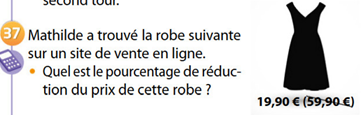
\includegraphics[scale=0.8]{ex37}
	\end{center}
	
	Une robe passe de \num{59.90} € à \num{19.90} €. \pause
	
	\begin{equation*}
		\num{59.90} - \num{19.90} = \num{40} 
	\end{equation*}

	La réduction s'élève à 40 €. \pause
	
	\begin{equation*}
		40 \div \num{59.90} \times 100 \approx \num{66.78} 
	\end{equation*}		
	
	Le prix de la robe a diminué de \num{66.78} \%.
\end{frame}


\begin{frame}
	\frametitle{Exercice 38}
	
	\begin{center}
		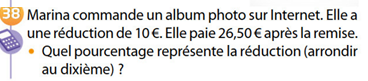
\includegraphics[scale=0.8]{ex38}
	\end{center}
	
	Un album coûte  \num{26.50} € après une réduction de 10 €.
	
	\begin{equation*}
		\num{26.50} + \num{10} = \num{36.50} 
	\end{equation*}
	
	Le prix de départ est \num{36.50}  €. \pause
	
	\begin{equation*}
		10 \div \num{36.50} \times 100 \approx \num{27.4} 
	\end{equation*}		
	
	Le prix de l'album a diminué de \num{27.4} \%.
\end{frame}

\begin{frame}
	%\frametitle{Exercice 58}
	
	\begin{columns}
		\begin{column}{0.5\textwidth}
			\begin{center}
				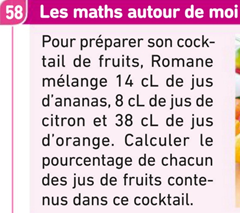
\includegraphics[scale=0.8]{ex58}
			\end{center}\pause
		\end{column}
		\begin{column}{0.5\textwidth}
			\begin{equation*}
				14 + 8 + 38 = 70
			\end{equation*}
		
		Il y a 60 cL de cocktail en tout. \pause
		
		\begin{equation*}
			14 \div \num{60} \times 100 \approx \num{23.3} 
		\end{equation*}		
		Il y a \num{23.3} \% de jus d'ananas dans le cocktail. \pause
		
		\begin{equation*}
			8 \div \num{60} \times 100 \approx \num{13.3} 
		\end{equation*}
	
		Il y a \num{13.3} \% de jus d'ananas dans le cocktail. \pause
		
		\begin{equation*}
			38 \div \num{60} \times 100 \approx \num{63.3} 
		\end{equation*}
		
		Il y a \num{63.3} \% de jus d'ananas dans le cocktail.
		
		\end{column}
		
	\end{columns}
	
	
	
\end{frame}


%\begin{frame}
%	\frametitle{Exercice 5 }
%
%	
%
%	
%	\begin{block}{{\centering Téléviseur $\frac{4}{3}$}}
%		\pause
%		\begin{eqnarray*}
%			\dfrac{Longueur}{largeur} &= & \dfrac{4}{3} \\ \pause
%			\dfrac{96}{?} &= & \dfrac{4}{3} \\ \pause
%			\dfrac{24 \times 4}{?} &= & \dfrac{4}{3} \\ \pause
%			\dfrac{24 \times 4}{24 \times 3} &= & \dfrac{4}{3} \\ \pause
%			\dfrac{96}{72} &= & \dfrac{4}{3}  \pause
%		\end{eqnarray*}
%		
%		Un téléviseur $\dfrac{4}{3}$ de 96 cm de longueur a une largeur de 72 cm. 
%	\end{block}
%
%
%	
%\end{frame}
%
%
%\begin{frame}
%	\frametitle{Exercice 31 page 77}
%
%	
%	
%	\begin{block}{Téléviseur $\frac{16}{9}$}
%		\pause
%		\begin{eqnarray*}
%			\dfrac{Longueur}{largeur} &= & \dfrac{16}{9} \\ \pause
%			\dfrac{96}{?} &= & \dfrac{16}{9} \\ \pause
%			\dfrac{6 \times 16}{?} &= & \dfrac{16}{9} \\ \pause
%			\dfrac{6 \times 16}{6 \times 9} &= & \dfrac{16}{9} \\ \pause
%			\dfrac{96}{54} &= & \dfrac{16}{9}  \pause
%		\end{eqnarray*}
%		
%		Un téléviseur $\dfrac{16}{9}$ de 96 cm de longueur a une largeur de 54 cm. 
%	\end{block}
%	
%	
%\end{frame}
%
%\begin{frame}
%	\frametitle{Exercice 51 page 79}
%	Le parcours fait 45 km.
%	
%	\begin{block}{Coureur 1}
%		\begin{eqnarray*}
%			d_1 &=& \frac{3}{2} \; de \; 45 \; km \\ \pause
%			d_1 &=& \frac{3}{2} \times 45 \\ \pause
%			d_1 &=& \frac{3 \times 45}{2} \\ \pause
%			d_1 &=& \frac{135}{2} \\ \pause
%			d_1 &=& \num{67.5}  \pause
%		\end{eqnarray*}
%	
%	Le premier coureur a terminé la course il a parcouru \num{67.5} km.
%	\end{block}
%\end{frame}
%
%\begin{frame}
%	\frametitle{Exercice 51 page 79}
%	Le parcours fait 45 km.
%	
%	\begin{block}{Coureur 2}
%		\begin{eqnarray*}
%			d_2 &=& \frac{4}{5} \; de \; 45 \; km \\ \pause
%			d_2 &=& \frac{4}{5} \times 45 \\ \pause
%			d_2 &=& \frac{4 \times 45}{5} \\ \pause
%			d_2 &=& \frac{4 \times 9 \times 5}{5} \\ \pause
%			d_2 &=& \num{36}  \pause
%		\end{eqnarray*}
%		
%		Le deuxième coureur a parcouru \num{36} km.
%	\end{block}
%\end{frame}
%
%
%\begin{frame}
%	\frametitle{Exercice 51 page 79}
%	Le parcours fait 45 km.
%	
%	\begin{block}{Coureur 3}
%		\begin{eqnarray*}
%			d_3 &=& \frac{7}{9} \; de \; 45 \; km \\ \pause
%			d_3 &=& \frac{7}{9} \times 45 \\ \pause
%			d_3 &=& \frac{7 \times 45}{9} \\ \pause
%			d_3 &=& \frac{7 \times 5 \times 9}{9} \\ \pause
%			d_3 &=& \num{35}  \pause
%		\end{eqnarray*}
%		
%		Le troisième coureur a parcouru \num{35} km.
%	\end{block}
%\end{frame}
%
%
%\begin{frame}
%	\frametitle{Exercice 51 page 79}
%		
%	\begin{block}{Bilan}
%		\begin{itemize}
%			\item Le premier coureur a terminé la course il a parcouru \num{67.5} km.
%			\item Le deuxième coureur a parcouru \num{36} km.
%			\item Le troisième coureur a parcouru \num{35} km. \pause
%		\end{itemize} 
%		
%		
%
%	\end{block}
%	
%	\vspace*{1cm}
%	C'est donc le premier coureur qui est en tête de la course.
%\end{frame}
%

\end{document}